\documentclass[letterpaper]{article}

% authors and affiliations
% \title{Correlated host movements can reshape spatio-temporal disease dynamics: modeling the contributions of space use to transmission risk using movement data}
% \usepackage{authblk}
% \author{Juan S. Vargas Soto, Justin Kosiewska, Lisa I. Muller, Daniel Grove, Dailee Metts, and Mark Q. Wilber}
% \affil{School of Natural Resources, University of Tennessee, Knoxville, TN}
% \date{}

\usepackage[english]{babel}
\usepackage[utf8x]{inputenc}
\usepackage{amsmath}
\usepackage{graphicx}
\usepackage[left=1 in, right=1 in, top=1 in, bottom=1 in]{geometry}
\usepackage{hyperref}
\usepackage{bbold}
\usepackage{rotating}
\usepackage{bbm}
\usepackage{array}
\usepackage{xcolor}
\newcolumntype{C}[1]{>{\centering\arraybackslash}m{#1}}
% \usepackage{kbordermatrix}
\usepackage{footnote}
\makesavenoteenv{tabular}
\makesavenoteenv{table}
% \renewcommand{\theequation}{{S}\arabic{equation}}

\makeatletter
% \addto\captionsenglish{%
%   \renewcommand{\fnum@figure}{Figure S\thefigure}%
%   \renewcommand{\fnum@table}{Table S\thetable}%
% }
\makeatother

% Bibliography
\usepackage[round, colon]{natbib} % Bibliography - APA
\bibliographystyle{abbrvnat}
%\bibpunct{(}{)}{;}{a}{}{,}

% Line numbers
\usepackage{lineno}
%\def\linenumberfont{\normalfont\footnotesize\ttfamily}
%\setlength\linenumbersep{0.2 in}
\linenumbers

% Set space
\usepackage{setspace}
\doublespacing

% Command to e.g. write code that doesn't show up. Used as \ignore {some code}
\newcommand{\ignore}[1]{}

\begin{document}


\noindent
\textbf{Title}: How do non-independent host movements affect spatio-temporal disease dynamics? Partitioning the contributions of spatial overlap and correlated movements to transmission risk

\bigskip

\noindent
%\textbf{Running title}: Temporal correlation reshapes disease dynamics

\bigskip

\noindent
\textbf{Authors}: Juan S. Vargas Soto\textsuperscript{1, a}, Justin Kosiewska\textsuperscript{1, b}, Lisa I. Muller\textsuperscript{1, c}, Dan Grove\textsuperscript{1, d}, Dailee Metts\textsuperscript{1, e}, and Mark Q. Wilber\textsuperscript{1, f}

\bigskip

\noindent
\textbf{Author affiliations}:

\noindent
\textsuperscript{1}School of Natural Resources, University of Tennessee Institute of Agriculture, Knoxville, TN \\
\textsuperscript{a} jvargass@utk.edu\\
\textsuperscript{b} jkosiews@vols.utk.edu\\
\textsuperscript{c} lmuller@utk.edu\\
\textsuperscript{d} dgrove@utk.edu\\
\textsuperscript{e} dmetts1@vols.utk.edu\\
\textsuperscript{f} mwilber@utk.edu

\bigskip

\noindent
\textbf{Corresponding author}: Juan S. Vargas Soto\\
Present address: School of Biological Sciences, Queen's University Belfast\\
19 Chlorine Gardens, Belfast BT9 5DL\\
Northern Ireland\\
j.vargas@qub.ac.uk
\bigskip

\noindent
\textbf{Acknowledgments}

Thanks to Dr. A. Houston, B. Trout, M. Turner and TWRA for capture and logistical support during fieldwork. Funding for this study was provided by the United States Department of Agriculture (USDA) National Institute of Food and Agriculture (McIntire Stennis project TEN00MS-113; Hatch Project 7001607) and the USDA American Rescue Plan (APP-21535). A portion of the computation for this work was performed on the University of Tennessee Infrastructure for Scientific Applications and Advanced Computing (ISAAC) computational resources.
\bigskip

\noindent
\textbf{Conflict of interest}: The authors declare no conflict of interest.

\bigskip
\noindent
\textbf{Author contributions}: JSVS and MQW conceptualized and developed the methods. JSVS performed simulations and analyses. JK led collection of animal movement data, assisted by DG, LM, DM, and MQW. JSVS wrote the first draft of the manuscript, and all coauthors contributed substantially to revisions. 

\bigskip
\noindent
\textbf{Data accessibility statement}: Data used in the manuscript, as well as code to generate simulations and analyze data, are available at on \url{https://github.com/juansvs/moveSTIR_collapse}. This repository will be archived on Zenodo upon acceptance.

\bigskip
\noindent
\textbf{Abstract}: XX words\\
\textbf{Main text}:  XX words\\
\textbf{References}: XX \\
\textbf{Figures and tables}: XX figures 

\newpage

\doublespacing
\linenumbers

\section*{Abstract} % 350 word limit for JAnEcol.  % You will probably want to restructure this slightly for JAE.  They use the numbered abstract structure.

1. Despite decades of epidemiological theory making relatively simple assumptions about host movements, it is increasingly clear that non-random movements drastically affect disease transmission. To better predict transmission risk, theory needs to simultaneously account for how the environment affects host space use and how social dynamics affect spatio-temporal correlation in host movements. 
2. We develop new theory that decomposes the relative contributions of fine-scale space use and correlation in space use to spatio-temporal transmission risk. We show analytically that, for directly transmitted parasites, even weak among-host correlations in space use can increase contact and transmission risk by orders of magnitude compared to independent movement. For this to hold, the area in which transmission occurs needs to be much smaller than the overall area individuals use -- a condition that is broadly true for many directly transmitted parasites. However, if the scale of transmission is substantially smaller than the scale at which social decisions occur, non-independent host movement plays almost no role for transmission risk even if hosts are highly correlated.
3. We provide a framework to estimate the FOI from empirical telemetry data, and use simulations to show that attraction between individuals can generate correlations in space use that greatly increase the risk of transmission, compared to independent movement. We apply this framework to GPS data from white-tailed deer, to infer the risk of transmission of two pathogens with widely different environmental persistence. We show for this empirical example how the effects of correlation scale up to multiple individuals, and how they could accelerate disease spread through a population. Our findings indicate that accounting for correlation is especially critical for directly transmitted pathogens with short environmental persistence. 
4. Our theory provides clear expectations for what has been observed empirically but largely ignored in disease models---movement correlation can reshape epidemiological landscapes, creating transmission hotspots whose magnitude and location are not necessarily predictable from spatial overlap alone.

\bigskip
\noindent
\textbf{Keywords}: transmission, contact, wildlife disease, spatial overlap, utilization distribution, animal movement

\section*{Introduction}

Individual movement is a critical factor influencing wildlife disease dynamics \citep{Dougherty2018,Manlove2022};
Movement determines encounters with other individuals of the same species, other species, or pathogens in the environment \citep{Martinez-Garcia2020,Das2023}. 
These encounters are necessary for the transmission of infectious diseases, and efforts have sought to identify where they occur, how often, and how they are influenced by environmental and social drivers \citep{Titcomb2021,Dougherty2022,Webber2023}. 
Formally linking social factors, environmental factors, animal movement, contact, and pathogen transmission would improve our ability to predict and prevent outbreaks and represent a significant advancement for management of wildlife diseases.  
Nevertheless, understanding how these processes interact at an individual scale requires detailed movement information and theory to translate movement into an epidemiological context.

Most epidemiological theory is built upon the assumption of independent host movements, and there is little theory that quantifies how non-independent, correlated movements affect contact and transmission risk. Despite empirical work quantifying how correlated and social movements can affect contact and transmission landscapes \citep[e.g.,][]{Kjaer2008,Grear2010,Schauber2015a}, we lack models that isolate the role of social interactions on spatio-temporal force of infection (FOI, the risk of transmission experienced by a host per unit time). This limits our ability to ask a key question for predicting spatio-temporal transmission risk on real-world landscapes: how do non-independent movements affect spatio-temporal infection risk, compared to spatial overlap?  In other words, under what conditions are patterns of animal space use sufficient for predicting contact and transmission and when do correlations in animal movements driven by social dynamics alter spatio-temporal transmission patterns relative to space use alone?  If correlations in animal movement generally have negligible effects on contact transmission once space use is known, then epidemiological landscapes can be largely predicted simply by understanding patterns of resource selection. However, recent studies have shown that spatial transmission risk can be highly localized \citep{Albery2021} and is not necessarily predicted by animal space use \citep{Yang2023a}. We hypothesize that non-independent animal movements can (at least partially) account for these observations and develop a modeling approach to rigorously test this hypothesis and systematically quantify the contribution of space use and non-independent movements to spatio-temporal transmission risk.

% Mark here:  Is this question and hypothesis clear enough?  We want to highlight this for JAE. Juan: I believe so,  I like the framing.

Recent developments at the interface of movement and disease ecology leverage high-resolution animal tracking data to gain insight into contact among individuals and disease transmission \citep{Richardson2015,Wilber2022,Yang2023}. For example, movement-driven spatio-temporal infection risk (MoveSTIR) builds dynamic contact networks from movement data to estimate individual risk of infection across space and time \citep{Wilber2022}. MoveSTIR provides a theoretical foundation to translate contacts into the epidemiological currency of FOI. These studies have highlighted the importance of individual heterogeneity and temporal scale for epidemiology, particularly how indirect contact---individuals at the same place at different times---can significantly reshape contact and transmission networks \citep{Richardson2015,Yang2023}. Current approaches are nonetheless based on occurrence, rather than range, distributions \citep[in the terminology of ][]{Alston2022} -- meaning they only consider where animals were and not where they \emph{potentially} could be. This approach makes it difficult to systematically link encounters with environmental drivers, and to predict how social or environmental changes affect contact and transmission.  Moreover, while MoveSTIR rigorously translates observed movement trajectories into metrics of epidemiological risk, it does not provide a way to partition the contributions of spatial overlap and non-independent host movements to epidemiological risk. Such a partition is needed to quantify and subsequently predict the ecological and epidemiological conditions where spatial and social drivers differentially affect transmission risk.

To address these limitations of MoveSTIR, it is useful to probabilistically consider spatio-temporal contact dynamics using utilization distributions (UDs). The UD represents the probability---transient or long-term \citep{Tao2016}---of an organism using some area \citep{Worton1989}. The high spatial and temporal resolution of modern tracking data serves to build UDs based on biologically realistic movement models \citep{Kranstauber2012,Fleming2014}, and to link them with underlying resources \citep{Potts2023}.
Additionally, combining individual UDs informs about pairwise interactions, by quantifying home range overlap \citep{Winner2018}, or estimating the expected location and rate of encounters \citep{Noonan2021}, which could serve to infer transmission risk \citep{Godfrey2010,Godfrey2013,Noonan2021} [Janine's paper]. 
Moreover, because UDs can be directly linked to environmental drivers of movement \citep{Signer2017}, they could be used for prospective analyses, to predict contact and transmission in novel environments, or to understand cascading effects of environmental and social perturbations from individual movement to population and landscape-level disease transmission.  Thus, UDs provide a general and intuitive method for i) linking contacts closely with environmental context (i.e., environment $\rightarrow$ UD $\rightarrow$ contact) and ii) predicting potential contacts beyond observed movement trajectories.

However, current contact metrics based on UDs have two limitations. First, they typically focus only on direct interactions, ignoring temporal dynamics related to indirect interactions that are especially relevant for epidemiological processes \citep{Yang2023}. Second, they consider independently moving animals, effectively assuming that any correlation in animal movement is unimportant for contact once space use is known. The Conditional Distribution of Encounters (CDE) \citep{Noonan2021}, for example, estimates local probabilities of encounter as a product of individual UDs, assuming that individuals move independently.
While a useful simplification, social interactions like territoriality or gregariousness can invalidate this assumption \citep{Manlove2018,Sah2018}. In these cases, temporal correlations in space use could increase or decrease the probability of encounter expected given independent movement \citep{Kjaer2008,Schauber2015a}. 
Moreover, direct interactions do not necessarily equate to \emph{epidemiological contacts}, which comprise contact formation and duration, as well as pathogen shedding, decay, and acquisition \citep{Herraiz2024}. As some pathogens can persist in the environment for months or years (e.g. anthrax, chronic wasting disease--CWD), ignoring these processes could severely underestimate transmission risk \citep{Wilber2022,Yang2023,Richardson2015}.  A comprehensive analytical framework is needed that combines utilization distributions, non-independent movements, and direct and indirect epidemiological interactions to quantitatively assess how these factors jointly shape spatio-temporal FOI and disease dynamics on real landscapes.

% The previously developed MoveSTIR implicitly accounts for such correlations, but only applies for observed data. In contrast, the CDE provides a basis for estimating encounter probabilities across the landscape, but ignores non-independent movements and temporal dynamics of indirect contact.
% To assess the role correlated movement can play of epidemiological landscapes \citep[\emph{sensu}][]{Manlove2022} an approach is needed that combines the range-distribution inference of UDs and CDEs \citep{Alston2022,Noonan2021} with the epidemiological focus of MoveSTIR to link UDs with epidemiological dynamics. 

Here, develop and apply a model we refer to as Probabilistic MoveSTIR (PMoveSTIR) to address a major knowledge gap at the interface of movement and disease ecology: under what ecological and epidemiological conditions do non-independent host movements affect spatio-temporal transmission dynamics?  We derive a general model that decomposes the contributions of transient, spatially heterogeneous UDs and a novel metric we refer to as the ``pairwise correlation surface'' that quantifies the contribution of non-independent host movements to spatio-temporal transmission risk. 
Deriving analytical results and applying PMoveSTIR to simulated data, we examine how the scale of pathogen transmission, the scale of host social decisions, pathogen persistence in the environment, and host movement patterns affect how non-independent host movements contribute to transmission risk.  However, the mismatches between the spatial scale of pathogen transmission and the spatial scale at which social decisions are made, as well as the duration of pathogen persistence in the environment, can drastically weaken the importance of correlated movements for transmission beyond space use. We apply our model to empirical movement data for white-tailed deer (\emph{Odocoileus virginianus}) and demonstrate on real movement data that non-independent movements can increase potential FOI by orders of magnitude for a hypothetical directly transmitted pathogen but are relatively unimportant for a hypothetical pathogen with long persistence times. Moreover, non-independent movements can yield highly heterogeneous transmission landscapes, supporting the emerging idea that fine-scale patterns of transmission dynamics are common in wildlife \citep{Albery2021} and are contributed to by correlated host movements. By precisely quantifiying the two fundamental components of non-random movements, fine-scale space use and correlation in movement, PMoveSTIR is a key next step for developing predictive models that link movement data to spatio-temporal infection dynamics on real landscapes.


\section*{Materials and Methods}

\subsection*{Model development - Review of MoveSTIR}

PMoveSTIR builds on the MoveSTIR model \citep{Wilber2022} and formally links UDs, direct and indirect contacts, non-independent movements, and spatial estimates of FOI. Essentially, we want to know, for two individuals $i$ and $j$ moving and interacting across a landscape, what is the expected FOI $i$ experiences from $j$, across space and time? 

As in MoveSTIR, we assume that transmission happens by an infected host depositing pathogen into the environment and another host picking that pathogen up. 
Deposition and acquisition can represent a range of processes, from coughing and inhaling in a matter of seconds, to depositing parasite eggs or larvae in the environment and another individual consuming these days or weeks later. 
Considering transmission through deposition and acquisition clearly links direct and indirect transmission along a continuum \citep{Wilber2022}, and it encompasses standard density-dependent transmission as a special case \citep{Cortez2021}. 

As derived in \cite{Wilber2022}, MoveSTIR defines the pairwise FOI host $j$ exerts on host $i$ in location $x$ at time $t$ as \citep{Wilber2022} (see Appendix X for a full derivation of equation \ref{eq:original_foi})
\begin{equation}
    h_{i \leftarrow j}(t, x) = \int_{-\infty}^{t} \underbrace{\beta'}_{\text{Acquisition}} \underbrace{\delta_{x_j(u)}(x)}_{\substack{\text{Contact:} \\ \text{$j$ in location $x$ at $u$}}}  \underbrace{\lambda \delta_{I_j(u)}(I)}_{\text{Deposition}} \underbrace{\Theta(t - u)}_{\text{Pathogen survival}} du
    \label{eq:original_foi}
\end{equation}
The term $x_j(u)$ is the location of individual $j$ at time $u$ and $\delta_{x_j(u)}(x)$ is an indicator function that is one if host $j$ is in location $x$ at time $u$ and zero otherwise. A location $x$ has some area $A_x$.  The parameter $\beta'$ is the rate at which host $i$ acquires pathogen within location $x$ and can be re-written as $\tilde{\beta} / A_x$, where $\tilde{\beta}$ can be considered a ``search efficiency'' term, with units area/time (e.g., $m^2 / day$), and $A_x$ gives the area of location $x$ where transmission can occur (henceforth the area of transmission). In equation \ref{eq:original_foi}, we assume that the likelihood of contact is uniform within location $x$ -- in other words, once two hosts are both within the location $x$, it no longer matters for contact how close they are to each other within this area \citep{Gurarie2013,Wilber2022}. Importantly, the area $A_x$ of location $x$ is a biological property of the pathogen and is separate from the movement ecology of the host. Area $A_x$ effectively defines how close individuals need to be before transmission can occur. While MoveSTIR considers different types of contacts based on the distance individuals are apart in continuous space \citep{Wilber2022}, here we assume that transmission occurs within grids on a landscape where the area of a grid cell $A_x$ is determined by the epidemiology of the pathogen of interest -- contact occurs when two individuals are in the same grid cell. How individuals move is independent of $A_x$, but how pathogens are transmitted depends on $A_x$.  While this grid approach is less general than a distance-based approach (see Appendix X), it is consistent with how many individual-based models capture direct or indirect transmission on landscapes \citep[e.g.][]{White2018e,Thompson2024} and also leads to many useful conceptual results.  

Returning to equation \ref{eq:original_foi}, the parameter $\lambda$ is the per capita pathogen deposition rate. We assume that $\lambda$ is constant and does not depend on time since infection. The variable  $\delta_{I_j(u)}(I)$ is an indicator function that is one if host $j$ is infected at time $u$ and zero otherwise.  The function $\Theta(t - u)$ is a pathogen survival function that gives the probability that pathogens deposited at time $u < t$ are still transmissible at time $t$.  

It is also useful to consider a consequence of some of our assumptions underlying equation \ref{eq:original_foi}. The parameter $\lambda$ is a per capita shedding rate and is not scaled by area. Over a unit of time, infected hosts will shed a finite amount of pathogen into the location $x$ that they are occupying.  Equation \ref{eq:original_foi} assumes that this pathogen instantaneously and uniformly fills the location $x$ such that there is a density of pathogen $\lambda dt / A_x$ in $x$ after $dt$ time units and no pathogen decay. 
As $A_x$ approaches zero, the deposited pathogen becomes infinitely dense and, because we assume there is no pathogen depletion upon acquisition, FOI goes to infinity.  While this limit is logically consistent with density-dependent transmission and no pathogen depletion, it is biologically nonsensical because a discrete host cannot occupy, shed, and acquire pathogen in an infinitely small area. Thus, there is a biological lower bound on $A_x$ that ensures that at least one host can fit into $x$. In what follows we will always consider that $A_x$ at minimum can encompass the depositing host and is often larger than the host (e.g., consider the 2m radius for transmission of the SARS-COV-2 virus during the COVID19 pandemic).

\subsection*{Model development -- Linking utilization distributions to transmission through PMoveSTIR}

We now derive the PMoveSTIR model from equation \ref{eq:original_foi}. First, we simplify equation \ref{eq:original_foi} by assuming that the depositing host is always infectious and shedding pathogen at a constant rate. This assumption is equivalent to building a contact network and also represents the structural form of FOI needed to compute pathogen invasion thresholds such as $R_0$ \citep[see][]{Wilber2022}.

Second, we consider probabilistic space use (i.e., we know where an individual is at a given time and location with some probability) and re-write equation \ref{eq:original_foi} as
\begin{equation}
    h_{i \leftarrow j}(t, x) = \int_{-\infty}^{t} \beta' \lambda \delta'_{x_i(t)}(x) \delta'_{x_j(u)}(x) \Theta(t - u) du
    \label{eq:prob_foi}
\end{equation}
where $\delta'_{x_i(t)}(x)$ is a random variable that specifies whether host $i$ is in location $x$ at time $t$ (defined equivalently for $j$).  This means that $h_{i \leftarrow j}(t, x)$ is also a random variable, and we can express its expected value as 
\begin{equation}
    h^*_{i \leftarrow j}(t, x) := E[h_{i \leftarrow j}(t, x)] = \int_{-\infty}^{t} \beta' \lambda E[\delta'_{x_i(t)}(x) \delta'_{x_j(u)}(x)] \Theta(t - u) du.
    \label{eq:expected_foi}
\end{equation}
Interpreting this expectation, we are asking: if we simulated some movement process thousands of times, what is the probability that host $i$ is in location $x$ at time $t$, and host $j$ was in $x$ at a previous time $u$?  While this is a simple mathematical extension to the MoveSTIR equation \ref{eq:original_foi}, it is a significant conceptual advance as it provides the mathematical structure necessary to link FOI directly with UDs and partition the contributions of spatial overlap and non-independent movements on FOI, as we describe next.

For two random variables $Y$ and $Z$, $E[YZ] = E[Y]E[Z] + Cov(Y, Z)$.  We can therefore write equation \ref{eq:expected_foi} as
\begin{equation}
    \begin{aligned}
        h^*_{i \leftarrow j}(t, x) &= \int_{-\infty}^{t} \frac{\tilde{\beta}}{A_x} \lambda E[\delta'_{x_i(t)}(x) \delta'_{x_j(u)}(x)] \Theta(t - u) du \\
        &= \frac{\tilde{\beta}}{A_x} \lambda \int_{-\infty}^{t} [E[\delta'_{x_i(t)}(x)] E[\delta'_{x_j(u)}(x)] + Cov(\delta'_{x_i(t)}(x), \delta'_{x_j(u)}(x))] \Theta(t - u) du \\
        &= \frac{\tilde{\beta}}{A_x} \lambda \int_{-\infty}^{t} [p_i(x, t) p_j(x, u) + Cov(\delta'_{x_i(t)}(x), \delta'_{x_j(u)}(x))] \Theta(t - u) du \\
    \end{aligned}
    \label{eq:foi_cov}
\end{equation}
where we use the fact that the expectation of an indicator variable is a probability \citep{Grimmett2001}. The terms $p_i(x, t)$ and $p_j(x,u)$ give the probabilities that host $i$ and $j$ are in location $x$ at times $t$ and $u$, respectively, and can also be written as $p_i(x, t) = \int_{A_x} f_i(k, t) dk$ where $f_i(k, t)$ is the probability density of host $i$ using the point $k$ at time $t$ and the integral is over the area of transmission $A_x$ (defined equivalently for host $j$). Thus, we have obtained an equation that links the transient utilization distributions $f_i(k, t)$ and $f_j(k, u)$ with the spatio-temporal FOI.
This general PMoveSTIR formulation accounts for heterogeneity in space and time, but the model can consider other scenarios, such as uniform space use or UDs that are stationary in time (Fig. \ref{fig:square}).  In terms of the novelty of equation \ref{eq:foi_cov}, we note that \cite{Wilber2022} in Appendix 9 considered a special case of PMoveSTIR looking at home-range overlap, but they did not link this equation to UDs and ignored covariance in movement.

A useful simplification of equation \ref{eq:foi_cov} considers that movement is statistically stationary in time. Equation \ref{eq:foi_cov} becomes (derivation in Appendix X)

\begin{equation}
    \begin{aligned}
    h^*_{i \leftarrow j}(x) = \beta' \lambda [ \underbrace{p_i(x)p_j(x) \int_0^{\infty} \Theta(s) ds}_{\substack{\text{FOI contribution from} \\ \text{spatial overlap}}} + \underbrace{\sigma_i(x) \sigma_j(x) \int_{0}^{\infty} Cor(\delta'_{x_i(k)}(x), \delta'_{x_j(k - s)}(x)) \Theta(s) ds}_{\substack{\text{FOI contribution from} \\ \text{non-independent movement}}}.
    \end{aligned}
    \label{eq:stationary_cor}
\end{equation}
The quantity $p_i(x)$ is the stationary probability of host $i$ using location $x$ and $\sigma_i(x) = \sqrt{p_i(x)(1 - p_i(x))}$ is the standard deviation in probability of host $i$ using location $x$ (defined similarly for host $j$). The term $Cor(\delta'_{x_i(k)}(x), \delta'_{x_j(k - s)}(x))$ is the (lagged) correlation between the occupancy random variables $\delta'_{x_i(k)}(x)$ and $\delta'_{x_j(k - s)}(x)$ for any time $k$ where the time lag is $s$.  Given the assumption of statistical stationarity, the correlation between the occupancy random variables of host $i$ and host $j$ does not depend on absolute time $k$ or $k - s$, but just the time lag $s$.   This is the quantity we refer to as the ``pairwise correlation surface''. Henceforth, we let $\rho(x ,s) = Cor(\delta'_{x_i(k)}(x), \delta'_{x_j(k - s)}(x))$. 

The pairwise correlation surface in equation \ref{eq:stationary_cor} is strongly related to the biology of host movements and the epidemiology of pathogen transmission.  A higher correlation term means that given host $i$ is in location $x$ there is a higher probability that host $j$ is also in location $x$.  For a correlation term equal to unity, when host $i$ is in location $x$ host $j$ is also in location $x$ with probability one.  Social interactions between hosts and the area of transmission $A_x$ will influence $\rho(x ,s)$.  For example, consider the extreme scenario where social interactions make it such that host $i$ and host $j$ are always 9 m apart, regardless of where they are on the landscape. If a pathogen can transmit between hosts when they are at most 10 m apart, then correlation is unity for all locations on the landscape. In contrast, if a different pathogen requires hosts to be at most 5 m apart for transmission, then the correlation is zero for all locations on the landscape. This emphasizes our previous point that $A_x$ is \emph{pathogen specific} and will influence the correlation term in PMoveSTIR.
% I'm not sure about this example, this applies if they are exactly 9 m apart, but that's not what we said. Also, in this scenario you could get rho=1 for some locations and rho<1 for others, depending on the distance, but we cannot claim that rho<1 for all locations. % Mark here: I think we actually can in What about this rephrasing? Juan: that works

Using equation \ref{eq:stationary_cor}, we can now ask: how much does the term $\sigma_i(x) \sigma_j(x) \int_{0}^{\infty} \rho(x, s) \Theta(s) ds$ contribute to FOI for different areas of transmission, social dynamics, and epidemiological scenarios? Specifically, throughout what follows we will focus on the ratio between non-independent movement contributions to FOI and spatial overlap (i.e., the correlation-spatial overlap ratio, $CSR(x)$): $CSR(x) = \frac{\sigma_i(x) \sigma_j(x) \int_{0}^{\infty} \rho(x, s) \Theta(s) ds}{p_i(x) p_j(x) \int_{0}^{\infty} \Theta(s) ds}$.  % Mark here: We need to use the same comparison throughtout.  I have been using this CSR term and you have been using something different.  I am fine with whatever metric, but it needs to be the same (the CSR metric is pretty simple to seems like a good one). Juan: yup fine by me

\subsection*{Analytical analysis: The effect of non-independent movements on FOI for uniform space use and direct contact}

Assume hosts are moving across a landscape of area $A_{tot}$. If they are using space uniformly, the probability of using any area $x$ with area $A_x$ is constant across space and among individuals, and we can update equation \ref{eq:stationary_cor} as

\begin{equation}
    \begin{aligned}
    h^*_{i \leftarrow j}(x) = \beta' \lambda [ \underbrace{\frac{A_x}{A_{tot}}\frac{A_x}{A_{tot}} \int_{0}^{\infty} \Theta(s) ds}_{\substack{\text{FOI contribution from} \\ \text{spatial overlap}}} + \frac{A_x}{A_{tot}} (1 - \frac{A_x}{A_{tot}})\underbrace{\int_{0}^{\infty} \rho(x, s) \Theta(s) ds}_{\substack{\text{FOI contribution from} \\ \text{non-independent movement}}}.
    \end{aligned}
    \label{eq:stationary_uniform}
\end{equation}
where we substituted $p_i(x) = p_j(x) = \frac{A_x}{A_{tot}}$ because both hosts are using space uniformly.  Moreover, $\sigma_i(x) \sigma_j(x) = \sqrt{\frac{A_x}{A_{tot}}(1 - \frac{A_x}{A_{tot}})}\sqrt{\frac{A_x}{A_{tot}}(1 - \frac{A_x}{A_{tot}})} = \frac{A_x}{A_{tot}}(1 - \frac{A_x}{A_{tot}})$.

Further, we assume that the pathogen survival function $\Theta(s)$ is a step function with a survival probability of one when lag $s \leq T$ and zero when $s > T$. With these assumptions, we can write equation \ref{eq:stationary_uniform} as

\begin{equation}
    \begin{aligned}
        h^*_{i \leftarrow j}(x) = \beta' \lambda \left[\frac{A_x}{A_{tot}}\frac{A_x}{A_{tot}} T + \frac{A_x}{A_{tot}}(1 - \frac{A_x}{A_{tot}}) \int_{0}^{T} \rho(x, s) ds\right],
    \end{aligned}
    \label{eq:uniform_stationary2}
\end{equation}

The correlation term $\rho(x, s)$ will be exactly $\rho(x, s = 0)$ when lag $s = 0$ (in words, $\rho(x, s = 0)$ is the correlation in two hosts' space use with a time lag of 0) and near $\rho(x, s = 0)$ when lag $s$ is near zero.  When pathogens are strictly directly transmitted, $T$ is small relative to the duration of time hosts spend in an area of transmission and we can reasonably approximate $\rho(x, s) = \rho(x, s = 0)$ from 0 to $T$.  We can then write equation \ref{eq:uniform_stationary2} as 
\begin{equation}
    \begin{aligned}
        h^*_{i \leftarrow j}(x) = \beta' \lambda T \left[\underbrace{\frac{A_x}{A_{tot}}\frac{A_x}{A_{tot}}}_{\substack{\text{Contribution due} \\  \text{to spatial overlap}}} + \underbrace{\frac{A_x}{A_{tot}}(1 - \frac{A_x}{A_{tot}}) \rho(x, s=0)}_{\substack{\text{Contribution due} \\ \text{to non-independent movement}}} \right].
    \end{aligned}
    \label{eq:uniform_direct}
\end{equation}
The $CSR(x)$ is simply 
\begin{equation}
    CSR(x) = (\frac{A_{tot}}{A_{x}} - 1)\rho(x, s=0)
    \label{eq:analytical_relationship}
\end{equation}

Before interpreting this equation, it is important to remember that $\rho(x, s=0)$ depends on $A_x$. The exact way that $\rho(x, s=0)$ scales with $A_x$ strongly depends on the movement strategies of the hosts.  While $\rho(x, s=0)$ is not fixed for $A_x$, we can reasonably look at how independently varying values of $A_x / A_{tot}$ and $\rho(x, s=0)$ affect the $CSR(x)$ because i) $\rho(x, s=0)$ is also driven by host parameters (e.g., mechanisms of social attraction) that are independent of $A_x$ (a pathogen parameter) and ii) $A_x / A_{tot}$ can change through $A_{tot}$ while $A_{x}$ remains constant.

Interpreting equation \ref{eq:analytical_relationship}, we see that when the area of transmission $A_x$ is small \emph{relative} to the total area that a host can occupy $A_{tot}$, even small levels of correlation $\rho(x, s=0)$ can result in non-independent movements having orders of magnitude larger contribution to FOI for direct transmission than spatial overlap (Fig. \ref{fig:analytical_corr}). This finding makes sense but is almost never considered in epidemiological models. If the area of transmission $A_x$ is small relative to $A_{tot}$ and hosts are moving randomly, there is a very low chance that hosts will be in an area of transmission together at the same time. Non-independent movements significantly increase this chance, even when correlation is low. In contrast, if a host's range is similar in size to the area of transmission (or more generally, if the probability of using a particular area is very high), then the importance of non-independent movement relative to spatial overlap becomes minimal (Fig. \ref{fig:analytical_corr}).  Given that transmission for many directly transmitted pathogens require hosts to be in relatively close contact, we would expect many empirical systems to be in the region where $A_x << A_{tot}$, meaning that even small levels of $\rho(x, s=0)$ can have significant effects on FOI compared to spatial overlap alone. 

\subsection*{Using simulations to test the contribution of non-independent movements to force of infection}

We considered two different simulations to gain additional insight into how non-independent movement influences local FOI. We use these simulations to explore the relative contribution of non-independent host movements for different scales of pathogen transmission $A_x$, scales of host social decisions, strengths of host social interactions, and rates of parasite decay.  We also use these simulations to examine our ability to actually empirically estimate the contribution of non-independent movements to FOI given limited movement data.

\subsubsection*{Simulation analysis, example 1}

In this simulation, we implement what we call a messy follow-the-leader model.  This is a strategic model that is geared to honing our intuition regarding the relative contributions of space use and non-independent movements to FOI. The steps in the model are as follows. There are some number of individuals on a landscape that have a strict social hierarchy -- individual 1 is dominant to individual 2, individual 2 is dominant to individual 3, as so on. Individuals can move between $N_h$ equal sized patches on the landscape, each with an area of 1. At each time step, dominant individuals move first, randomly selecting the next patch to move to. Any subordinate individuals that were in the same patch will either follow the most dominant individual with probability $p_f$, or select a random patch with probability $1 - p_f$.

The area of transmission is assumed to be smaller than the 1 unit area of the patches where social dynamics and movement decisions occur. Specifically, the area of transmission for a pathogen is $1 / N_p$ of the area of a habitat patch.  For simplicity, one can envision $N_p$ grid cells comprise each habitat patch and transmission can happen when two hosts in the same patch are also in the same grid cell. Once in a patch, we assume that individuals are also randomly located within the patch. Under these conditions, non-independence in movement may result in epidemiologically relevant correlation in space use, but this will depend on the relative size of the grid cells and the patches. 

Given this model, we ask: What is the relative contribution of non-independent movement to FOI compared to spatial overlap for hosts moving and interacting in this model and how does it depend on the scale at which social decisions are made?

\subsubsection*{Simulation analysis, example 2: Continuous-time movements and the effects of correlation on direct and indirect transmission}

Our second simulation mimics empirical trajectories obtained with telemetry methods, where movement is continuous in space but positions are obtained at discrete time points. We simulated two individuals that moved across the landscape following an Ornstein-Uhlenbeck process. In animal movement ecology, this process is used to represent Brownian motion restricted to a finite home range \citep{Hooten2017a, Blackwell1997}. Trajectories are created as an iterative process, at each step, an individual's coordinates are updated according to % Mark: Add citation here for OU process. Maybe Balckwell. Juan:added Blackwell
\begin{equation}
	x_i(t+1)=x_i(t)-\frac{1}{\tau}(x_i(t)-x_{\Omega,i})+\sqrt{\gamma}\epsilon
\end{equation}
% Mark here: We should probably write this in multivariate form or explicitly state that are we are assuming no correlation among x and y coordinates.
where $1/\tau$ represents the degree of attraction to the home range center $x_{\Omega,i}$, $\gamma$ is a diffusion parameter that defines the scale of movement, and $\epsilon$ is a random value from a standard normal distribution that drives the Brownian motion component. x and y coordinates are updated separately, effectively assuming no correlation between them. 

% Mark here:  You will probably want to provide more explantation of this in the appendix.  Actually give the equations or psuedo code. Juan: Ok will add to SI
To create different levels of correlation in space use, we modified the initial simulated trajectories using a convolution approach \citep[][, Appendix XX]{Scharf2018}. In the case of two individuals, this modification amounts to shifting the positions of individuals $i$ and $j$ at a given time $t$ closer together. At each time step, modified coordinates are calculated as the dot product of a social interaction kernel and the original coordinates. The elements of this kernel can be considered ``interaction strength'' terms, with values between 0 (no change to the original positions) and 1 (positions become identical). We assumed a constant, symmetric, and positive interaction strength (we do not consider repulsion because it has the same behavior as independent trajectories), although the convolution approach allows to relax these assumptions. In these simulations, local correlation in space use is an emergent property determined by the interaction strength, the area of transmission $A_x$, and the underlying movement process. 

We tested 7 different interaction strengths between 0 and 1, and performed 20 simulations for each one, each simulation lasting 3 weeks (500 1 h steps). Movement parameters were the same across all simulations, so individual home range sizes were similar across individuals. Every simulation had a different pair of home range centers with coordinates drawn randomly from a Poisson distribution. % Mark here: Confused here.  Do you mean Poisson process?  A poisson distribution would given discrete locations, but space is continuous.  Also, you are persumably drawing x and y? I assume these are uncorrelated in the draw? Juan: Yes all coordinates are uncorrelated, but drawn from the same distribution. It is actually a Poisson distribution, so you do get integer coordinates. This is only for the start of the simulation though, and because of the scale (10^2) it really makes no difference whether they are integers or not.

We used equation \ref{eq:stationary_cor} to compute the contributions of non-independent movement and spatial overlap to FOI.  Specifically, we let the pathogen survival function $\Theta(s) = \exp(-\nu s)$, where $\nu$ is the rate of pathogen decay. For every simulation we calculated multiple FOI values, using different possible combinations of pathogen decay rate $\nu$ (1/2 hours - 1/7 days) and area of transmission $A_x$ (1 m$^2$, 25 m$^2$, 100 m$^2$). %  Mark here: Should we give more information here on exactly how the each component of equation \ref{eq:stationary_cor} was estimated? How did we estimate UDs and how did we estimate the correlation surface?  Maybe just refer to the figure?

The pairwise correlation surface may vary as individuals use more of the space, or revisit past locations. To investigate how this affects FOI and the relative effect of correlation, we conducted longer simulations (1000, 2500, and 5000 steps, [where a step is 1 hr]) and recalculated the FOI. 

\subsection*{Empirical application - White-tailed deer}

To test the role of spatial overlap and non-independent movements on potential transmission risk in a real system, we applied the PMoveSTIR model to GPS-tracking data for five white-tailed deer from Ames Plantation, Tennessee, USA (one adult male and four adult females). 
Deer were captured and equipped with GPS collars that recorded fixes every 30 minutes (Lotek LiteTrack Iridium 420, Newmarket, Ontario, Canada; IACUC \# 2850-1021).  All individuals used in this study were captured at the end of March 2023 but we only included movement data from May to June in this study, to eliminate any effects of capture. 
%Similar to the simulations, we used CTMM and AKDE to estimate individual UDs \citep{Calabrese2016}. We estimated a median home range size of 0.6 km2.  We used the CTMMs to interpolate the positions to regular 10-minute intervals \citep{Yang2023}. We assumed a threshold contact distance of $d = 10 \text{ m }$ and an area of transmission of $A_x = 100 \text{ m}^2$.

We modeled two hypothetical pathogens. The first pathogen had a relatively short persistence time in the environment, surviving for an average of 1 hour  ($\nu=1\text{ h}^{-1 }$). In this case, transmission is largely direct and this might represent a pathogen like SARS-COV-2, which can infect and transmit between white-tailed deer \citep{Hale2022}. The second hypothetical pathogen had a long persistence time, remaining viable for over a year on average ($\nu=0.9 \text{ yr }^{-1}$). In this case, transmission is largely indirect and might reflect a pathogen like CWD, which can transmit directly and indirectly between deer and can persist for years in the environment \citep{Saunders2012a}. The $\beta'$ and $\lambda$ parameters are scalars in PMoveSTIR and do not affect any relative comparisons, so we set them both to unity. %As in the simulations, we pre-whitened and filtered correlation values to remove potentially spurious correlations. 
We used these data to explore how differences in overlap across home ranges and correlated movement influence the expected FOI with real animal trajectories, and how this would scale up to disease spread through a network of multiple individuals. To characterize disease spread across the population, we estimated relative $R_0$ values for a simple Susceptible-Infected-Recovered model, using three transmission matrices, one with the FOI estimated using correlation, one with the FOI without correlation, and one with home range overlap.  % Mark here: Let's show this in the appendix or reference Wilber et al. 2022. 

We followed the process described in Fig. X to quantify FOI from the trajectories for simulation 2 and for the deer trajectories. This process involves calculating the quantities of equation \ref{eq:stationary_cor} -- namely, the stationary utilization distributions for each individual and their correlation in space use.  To calculate the utilization distributions, we fitted continuous-time movement models (CTMM) to the trajectories, and estimated individual UDs using autocorrelated kernel density estimation (AKDE), as implemented in the ctmm R package \citep{Fleming2014, Calabrese2016,Fleming2022}. CTMMs model animal movement as a continuous process independent of sampling interval, and are therefore the tool of choice for reconstructing trajectories and estimating space use from telemetry data \citep{Fleming2014}. We gridded our landscape into areas of transmission $A_x = 100 \text{m}^2$ (i.e., 10m by 10m grids) and used the AKDE to calculate the probability of use in each grid for each host.    % Mark here: Great, should we say this above? 
%We used these methods to mimic how we might estimate UDs from real movement data where the underlying movement-generating process is unknown. 
%Kernel density estimation methods discretize UDs across a grid, here we set this grid to be composed of square cells with side $d$ equal to the approximate threshold contact distance for epidemiological contact. %We used the UDs to calculate the product of the probabilities of use ($p_i(x)p_j(x)$) and the product of their standard deviations ($\sqrt{p_i(x)(1-p_i(x))}\sqrt{p_j(x)(1-p_j(x))}$) as given in equation \ref{eq:stationary_cor}.


To calculate an approximation to pairwise correlation surface, we created individual position histories. The position history for each individual is a binary matrix, where rows represent discrete time steps and columns represent cells, that shows whether each individual was present or absent at time $t$ at location $x$ (Fig. X). We used the CTMMs to interpolate deer positions to regular 10-minute intervals \citep{Yang2023} to ensure rows matched across individuals, and that there were no missing entries in the position histories. Calculating the cross-correlation between corresponding columns of the matrices gives the local correlations across multiple lags. %This calculation is performed for discrete times, which in the case of empirical data required interpolating the positions to common time points. The cross-correlation can only be calculated at locations that both individuals visited. Locations that only one or neither individual visited have empirically unknown correlations that we conservatively set to zero. 
 %The order of visits matters, so correlation values can be asymmetric between individuals. 
Correlations can appear spuriously as statistical artifacts, even in the absence of a true biological interaction (i.e., interaction strength $=0$).  The reason for this related to our theory and simulations above -- very small values of correlation in an area can matter a lot for transmission relative to space use, but estimating correlation values with sufficient precision from finite movement data is difficult.  Therefore, we can only reliably estimate the contributions of correlation in locations where correlation is sufficiently large as to not run into issues with precision and statistical power. To address this issue, we effectively set all potentially spurious correlation to zero to be conservative with regards to how much correlation might be affecting FOI relative to space use. 

Specifically, we first performed a pre-whitening step to remove the potential effects of autocorrelation on cross-correlation. Pre-whitening consists of fitting an autoregression model to one of the series, and filtering both time series using the coefficients from that model \citep{Dean2016}. Additionally, we retained only correlation values deemed significantly different from 0, i.e. correlations with absolute values greater than a threshold of $1.96/\sqrt(N)$, where $N$ is the length of each time series \citep{Dean2016}. All other values were set to 0 as they are considered random noise. 

We scale each retained correlation value by the exponential pathogen survival function $\Theta(s) = e^{-\nu s}$, where $s$ is the lag corresponding to each cross-correlation, and $\nu$ is the decay rate of the pathogen in the environment. This assumes immediate transmissibility following deposition and a constant decay rate. Integrating across lags gives a single decay-weighted correlation value for each grid cell considered. In our implementation, times are discrete, so instead we multiplied each value by $ds$, the interval between successive positions, and added the results together. To obtain the per-cell FOI, we substituted the terms in equation \ref{eq:stationary_cor} and scaled by the epidemiological parameters $\tilde\beta\lambda/ A_x$. As a comparison point, we calculated a correlation-independent FOI, considering only product of the UDs, which effectively assumes independent movement. We averaged both over all grid cells on the landscape, and quantify the relative influence of correlation as the ratio between the two FOI values. % Mark here: Let's make sure we use the same comparison of contribution throughout. Either this metric or CSR = Correlation / Spatial overlap. Juan here: Yes, I've changed the figures to reflect CSR. 

\section*{Results}

\subsection*{Simulation study 1}

The messy follow-the-leader model has an analytical solution for correlation in movement for any two individuals at a time lag of 0 that is given by (Appendix X)
\begin{equation}
    \rho_{messy}(x, s=0) = \frac{p_f(N_h - 1)}{(n_p N_h - 1)(N_h(n_p - p_f) + p_f)}.
    \label{eq:messy_leader}
\end{equation}

The $CSR(x)$ is
\begin{equation}
    CSR(x) = \frac{\frac{1}{N_h n_p}(1 - \frac{1}{N_h n_p})\rho_{messy}(x, s=0)}{\frac{1}{N_h n_p} \frac{1}{N_h n_p}} = \frac{p_f(N_h - 1)}{N_h(n_p - p_f) + p_f}.
    \label{eq:relative_contrib}
\end{equation}

Equation \ref{eq:relative_contrib} highlights two keys results.  First, if the area of transmission $A_x = 1 / n_p \leq 1 / 2$ (i.e., the area of transmission is half the size or less compared to the area over which hosts are making social decisions), then the contribution of non-independent movement to FOI can at most be equal to the contribution from spatial overlap. This happens when $N_h$ is large and $p_f = 1$ (equation \ref{eq:relative_contrib}, Fig. \ref{fig:follow_the_leader}A). As $1 / n_p$ goes to zero, the $CSR(x)$ goes to zero regardless of the probability of following the leader $p_f$ (Fig. \ref{fig:follow_the_leader}A). In other words, if the social decisions are happening at a scale substantially larger than the pathogen's area of transmission, then from the pathogen's perspective hosts are moving randomly and correlation in movement does not matter for FOI.  Moreover, even if the area of transmission is half the scale at which social decisions take place, non-independent movements will generally matter less than spatial overlap for FOI. 

Second, in stark contrast to the above result, if social decisions are happening at a similar scale as the area of transmission ($n_p = 1$), then there is always some $p_f$ for which non-independent space use will have a higher contribution to FOI compared to spatial overlap (Fig. \ref{fig:follow_the_leader}A).  For example, as $N_h$ gets very large and $n_p = 1$, meaning that the total area that hosts move on the landscape is large relative to the area of transmission, the $CSR(x)$ approaches $p_f / (1 - p_f)$. If $p_f$ is greater that 0.5, then non-independent movement will matter more than spatial overlap for FOI, otherwise non-independent movement will matter less than spatial overlap (Fig. \ref{fig:follow_the_leader}A). 

These results support the general equation \ref{eq:uniform_direct} and Figure \ref{fig:analytical_corr}, highlighting that even small levels of correlation in movement can significantly increase FOI relative to spatial overlap alone. For example, consider $n_p = 1$, $N_h = 10000$ and $p_f = 0.9$.  The pairwise correlation surface is $\rho_{messy}(x, s=0) = 0.00089)$ and the conditional probability of one host being in a patch given another host is in a patch is 0.00099. However, non-independent movement contributes nine times more to FOI than spatial overlap alone.  This result also has important empirical implications that we will return to in the next section -- a system could potentially have levels of correlation that are practically inestimable from a finite amount of movement data, yet this amount of correlation could still be driving observed spatio-temporal transmission dynamics.


\subsection*{Simulation study 2}

%The overall FOI varied more than four orders of magnitude among simulations, in response to both movement and epidemiological parameters. 
\subsubsection*{Effect of correlated movement on pairwise FOI}

In our more ``realistic'' simulations, greater interaction strengths were associated with higher spatial overlap among home ranges, but there were also pairs moving independently with similarly high  ($>$0.9) overlap. 
These scenarios allowed us to compare the FOI while teasing apart the effects of spatial overlap and non-independent movements. 
The FOI was higher for pairs with higher interaction values (i.e. with stronger attraction), in part due to the resulting increase in spatial overlap. 
However, we saw an even greater increase in FOI when we accounted for temporal correlation, and the difference between the two increased with higher interaction strengths (Fig. \ref{fig:simresults}a). For very strong interactions (strength$>$0.9), the FOI with correlation was more than ten times the FOI estimated without correlation, and there was a more than 100-fold difference for perfectly overlapping trajectories.  

% Methods that ignore temporal correlation could therefore be significantly underestimating transmission risk. 

%The FOI was generally greater when we accounted for correlation; in only 19\% of cases the estimates were equal with or without correlation, and in no instance was there a decrease. This effect is to be expected as we only included attraction in the simulations. 
We found that correlation could increase the estimated FOI even for pairs that moved independently, with an interaction strength of 0. In some cases the contribution of correlation to FOI could be as much as six times greater than the contribution from shared space use, and this effect was more likely for pairs with higher spatial overlap (Fig. \ref{fig:simresults}b). %While this was generally rare (86\% of cases had less than 20\% increase), there were  instances where the estimated FOI was more than three times greater.
Thus, even when there is no process of attraction, substantial overlap in home range can lead to apparent correlation in local space use.%While the expected correlation is 0 when individuals move independently, joint space use could lead to apparent correlations, especially when there are few observations in a given cell. 
These correlations can persist after pre-whitening and removing the majority of statistically spurious correlations. Apparent correlations are important to consider when analyzing empirical data where the true correlation and the degree of attraction/avoidance among individuals are unknown. Temporal reshuffling methods such as those proposed by \citet{Spiegel2016} can be a useful tool to establish the baseline ``apparent'' correlations that appear for non-socially interacting individuals. 

\subsubsection*{Influence of epidemiological parameters}

The FOI ratio was inversely proportional to mean decay time, meaning the relative contribution of non-independent movements is greatest for pathogens with shorter survival times (Fig. \ref{fig:simresults}d). While longer pathogen survival times increase the probability of indirect epidemiological contact, the expected rate of encounter at longer lags approximates the expected rate of encounter under independent movement, so correlations at long lags have only a small modifying effect on the expected FOI. % Mark here: Do you we just leave it at that?  Or do we want to say something about how high autocorrelation in movement will make non-independent movements matter more for FOI and indirect contact? Juan: Maybe, but we don't have that result clearly shown in these simulations. 

The effect of transmission distance on FOI--represented here by the size of the grid cells--depended on interaction strength and the effect of correlation (Fig. \ref{fig:simresults}c). Consistent with our analytical results, when animals are highly correlated in their movements (i.e., have a high interaction strength) the importance of non-independent movements is diminished as the area of transmission increases (Fig. \ref{fig:simresults}c).
However, our simulations also show that for non-perfectly overlapping individuals, larger areas of transmission can increase the probability of finding two individuals in the same cell sufficiently to offset the inherent reduction in transmission in larger areas (remember, $\beta' = \tilde{\beta} / A_x$), therefore increasing the relative contribution of correlation to FOI for trajectories that are already close in space.

\subsubsection*{Influence of data availability}

With longer time series, the number of cells that both animals visited (where correlation is calculated) increased linearly. This resulted in greater overall FOIs. However, the average FOI ratio in cells that both animals visited was relatively uniform...   % Mark here: Instead of overall FOI, we probably should be calculating mean per cell FOI conditional on use.  That way we are not confounding anything with number of cells used. Juan: makes sense
with more tracking data (Fig. \ref{fig:simresults}e), although local correlation values could decrease. 
Since we did not include any environmental drivers of movement, the expected correlation should be similar across the landscape. 

The cumulative correlation, however, is not related to the product of either the UDs or the standard deviations. This result highlights the challenge of predicting an expected correlation based on currently used metrics of movement and space use.

%Getting more data means that the correlations at the local (cell) level become more accurate, and that the correlation can be estimated for more locations. %Empirical movement studies should therefore try to ensure that the tracking duration is sufficient for the animals to cover the majority of their home range, so that estimated correlations are representative of the true underlying relationship. Given the complexity of the correlation, which may be determined through a combination of environmental factors and specific social interactions, predicting the underlying correlation surface could prove quite challenging. 

\subsection*{Empirical example: white-tailed deer}

The total potential FOI % Mark here: Could we instead do average per cell FOI conditional on use? Juan: Sure, I'll rerun the analyses.
varied more than six orders of magnitude across pairs of deer, partially due to differences in home range overlap, which ranged between 0 and 90\% (Bhattacharyya coefficient; Fig. \ref{fig:empiricalres}). While higher overlap generally correlated with higher FOIs, we estimated higher values when we accounted for correlation in movement, and the difference was not necessarily related with overlap (Fig. \ref{fig:empiricalres}a-c).  For the pair with the highest spatial overlap, the FOI was more than ten times greater when we accounted for correlation. Temporally reshuffling the trajectories of these individuals  \citet[following ][]{Spiegel2016} confirmed that this increase in FOI due to correlation was far beyond what we would expect from any  spurious, ``apparent'' correlations that could arise in independently moving hosts (as identified in our simulations). For all pairs considered, ignoring correlation could result in between 5\% and 96\% underestimation of FOI (under our assumptions about pathogen decay function and rate). These effects of correlation on FOI were strongest for pathogens with a fast decay rate. For a pathogen like CWD that can persist for very long in the environment, the FOI was virtually identical with or without correlation in host movement (Fig. \ref{fig:empiricalres}c). 

Given the localized nature of interactions, the changes in overall estimated FOI are caused by increases at particular cells. Consequently, the estimated FOI is heterogeneous across the landscape (Fig.\ref{fig:empiricalres}b). % Mark here: I am curious how much we want to emphasize this point given we have a better sense of how much finite movement data can drive the observed heterogeneity? Alternatively, intead of showing a spatial map, could we just focus on the points of high use and who the heterogeneity in FOI among these points?  That would still make this point but we wouldn't be biased by the spatial map looking really heterogeneous because we don't observe any points in a lot of locations. Juan: Hmm that's a good point.
These effects at the local and individual scale affect population-level pathogen transmission. For example, given a simple Susceptible-Infected-Recovered model and short pathogen persistence time in the environment, the relative $R_0$ on our network of five individuals was more than ten times greater when we accounted for correlation (Fig. \ref{fig:empiricalres}d). Thus, we would predict more explosive transmission through a network that considers fine-scale space use and correlation compared to one that assumes independent movement.

\section*{Discussion}

We develop a new model, PMoveSTIR, that disentangles the contributions of spatial overlap and correlated space use to spatio-temporal contact and transmission risk. Our results provide clear expectations for what has been previously observed empirically but largely ignored in movement and disease models -- correlation in movement can reshape epidemiological landscapes, leading to hotspots of transmission whose magnitude and location are not necessarily predictable from models of joint space use, in particular for directly transmitted or short-lived pathogens.  
%We linked our theory to standard mean-field population models in disease ecology to analytically show how even weak correlations in movement between pairs on the landscape can significantly alter population-level disease dynamics compared to standard assumptions of independent movement.
%PMoveSTIR explicitly emphasizes processes relevant for transmission, such as contact---direct and indirect---among individuals, pathogen shedding and survival in the environment, and, importantly, correlation in space use.  This framing sets our model apart from recent developments for inferring contact, which focus only on direct encounters and assume hosts move independently \citep{Noonan2021,Das2023}. This assumption can significantly underestimate transmission risk, with consequences for inferred disease spread across the population.
PMoveSTIR provides a clear, quantitative guide to assess when fine-scale, temporally synchronous movement data are necessary for capturing disease dynamics and when coarser scale, asynchronous data focused strictly on UD estimation are sufficient. 
In particular, we show that correlation in movement and synchronicity can be critical aspects of transmission for faster-paced pathogens, i.e. pathogens with short environmental persistence and transmission driven by short-term contacts \citep[cf.][]{Dougherty2018,Manlove2022}, such as canine distemper virus, rabies, or SARS-COV-2 (SCV2). 
SCV2 is of particular public health interest and recent studies have shown that it can infect a wide-range of wildlife hosts, including white-tailed deer \citep{Palmer2021,Hale2022}. There is also evidence that white-tailed deer can transmit SCV2 between each other in controlled experiments and in the wild \citep{Martins2022,Hale2022}, suggesting SCV2 can successfully invade, spread, and persist in wildlife.  In our analysis of empirical white-tailed deer movements, we found that ignoring correlation in movements and focusing only on patterns of space use led to a ten-fold change in $R_0$ for a SCV2-like pathogen on even a simple network, with significant implications for pathogen spread.  In contrast, our simulation and empirical results show that correlation may only have marginal effects on transmission of pathogens with longer persistence times like CWD and anthrax, and joint space use would be largely sufficient for understanding local transmission risk.


% Interestingly, transmission patterns of CWD in white-tailed deer only partially support this finding, as increased genetic relatedness (a proxy for social connectedness) increased the probability of infection beyond shared space use \citep{Grear2010}. Given the complex relationship between animal movements and time-lagged correlations (Fig. S1), there could be scenarios where correlations or direct contacts can disproportionately affect transmission risk even for pathogens with long environmental persistence.  PMoveSTIR provides a theoretical foundation to explore these scenarios in future studies.

Correlations in space use that are not accounted for by UDs typically reflect social interactions, for example herding animals, parents with their offspring, or mates temporally moving together \citep{Scharf2016,Yang2021}. 
White-tailed deer female groups, for example, have high social affinity. Thus, pairs of deer with equivalent habitat overlap have substantially higher contact rates when both individuals are within the same social group \citep{Schauber2007a,Kjaer2008,Schauber2015a,Grear2010}. This is likely the case in our empirical study; the pair with the greatest home range overlap and potential FOI was a mother--daughter pair. The overlap and interaction among them is consistent with the rose petal hypothesis \citep{Porter1991}, in which the home ranges of offspring radiate around the home range of their parent. The potential FOI in this case was over 10 times greater than for other pairs, despite similar degrees of habitat overlap. Importantly, 91\% of the total FOI (for a hypothetical directly transmitted pathogen like SCV2) would be missed if we only considered overlapping UDs for these individuals \citep[e.g., using a metric like CDE][]{Noonan2021}. While the importance of social interactions for contact rates has been documented previously in white-tailed deer \citep{Grear2010,Schauber2015a}, PMoveSTIR allows us to directly quantify the contribution of these social interactions to the FOI and move from qualitative conclusions to movement-informed quantitative models of disease invasion.

In practice, however, correlations influencing FOI may arise from fine-scale temporal patterns of resource use unrelated to social interactions. For instance, consider two individuals independently visiting a common resource at similar times \citep[e.g., a watering hole,][]{VanderWaal2017}. If the resource is highly localized in space and time, the joint, stationary UD would not necessarily predict this as an area of high contact and transmission risk. Rather, observed contacts in this area would be associated with correlation in movement and not long-term, predicted space use.
Alternatively, temporally varying UDs (i.e., the top right corner in Fig. \ref{fig:square}) would correctly capture that the joint occurrences were a result of spatio-temporal patterns of space use, reducing the relative importance of correlations on FOI. Unfortunately, non-parametrically estimating transient UDs at fine temporal scales with limited data points is not often feasible. Therefore, while the correlation term of PMoveSTIR will remain crucial to capture epidemiologically important spatial correlations in movement, it does not always provide an exact separation between spatial and social factors driving transmission risk.


A broad goal of PMoveSTIR is to create an epidemiological risk landscape independent of geographical location \citep{Merkle2018,Manlove2022}, which could be achieved by linking movement data and inferred contact with underlying environmental factors. Establishing these contact-environment links could enable out-of-sample prediction of transmission risk, for example to forecast future disease dynamics in the study population, project population-wide disease spread as information on more individuals becomes available, or quantifytra transmission risk for other populations in similar environments. Our model provides a generalizable theoretical foundation to perform similar analyses across different host-pathogen systems, and it can be integrated with any UD estimation method \citep{Signer2017,Merkle2018,Michelot2020,Potts2023}. In addition to movement covariates, PMoveSTIR can also incorporate spatially and temporally heterogeneous epidemiological parameters, for example pathogen survival rates that vary between habitats and seasons \citep{Daversa2017}, or spatially localized shedding \citep{Weinstein2018a}.

% Previous studies have created system-specific models that make this link, for example using probabilities of use informed by step selection functions with environmental covariates to simulate local disease dynamics \citep{Merkle2018}.

A key challenge for making out-of-sample predictions is empirically estimating the correlation surface.  While this term is well-defined in theory (equation \ref{eq:stationary_cor}), finite movement data can inherently only provide a patchy view of the true correlation surface (e.g., Fig. \ref{fig:steps}).  Our simulations showed that when animals were experiencing known social attraction at a time lag of zero, empirically estimated spatial correlations underestimated the contribution of correlation to FOI. This underestimation is not surprising because, without interpolation, we are limited to analyzing correlations where joint occurrences were observed and not where they potentially could have occurred. We did not use spatial interpolation tools (e.g., Kriging from a spatially-explicit statistical model, Clough-Tocher 2D interpolators, etc.) so our estimates provide a conservative view of how correlation could reshape epidemiological landscapes.  To adequately predict transmission landscapes out-of-sample, future work will need to develop robust approaches for estimating and predicting the entire correlation surface. 

Predicting epidemiological landscapes from host movements relies on the key assumption that environmental characteristics strongly influence movement and space use. While there is a growing number of methods that quantify the effect of environmental characteristics on movement and habitat use \citep[reviewed in][]{Hooten2017a}, there has been much less work exploring how (and if) environment affects and predicts correlation and synchrony among hosts.  Therefore, an essential next-step for building epidemiological landscapes will be predictive models of spatio-temporal correlation among individuals \citep[e.g.][]{Brandell2021}.
Our analyses emphasize the importance of this next step by showing that correlations at a local (cell) scale can create a vastly more heterogeneous transmission landscape. Moreover, correlations can lead to localized transmission hotspots that are not necessarily predictable from joint space use \citep{Yang2023a}, and may contribute to the growing empirical recognition that fine-scale, localized transmission hotspots are present in many empirical host-pathogen systems \citep{Albery2021}.  Whether these localized transmission hotspots are predictable \emph{a priori} remains to be seen, but ignoring non-independent movements can make the task orders of magnitude more difficult for some pathogens.

%\bibliographystyle{amnat.bst}
\bibliography{references.bib}

\clearpage

\begin{figure}
    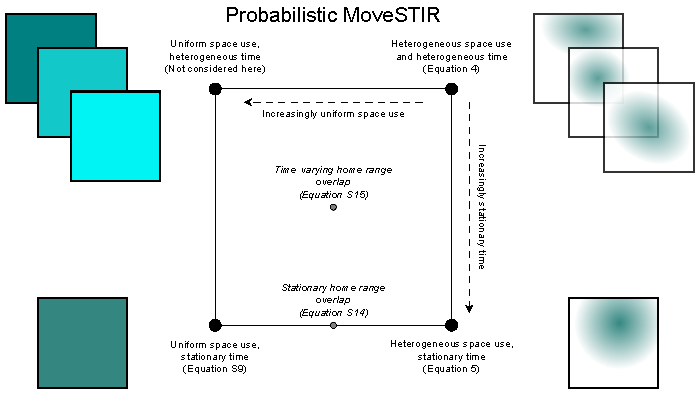
\includegraphics[width=\textwidth]{figures/conceptual_figure_pmovestir_mod.pdf}
    \caption{Conceptual figure describing the model developed in this manuscript: probabilistic movement-driven modeling of spatio-temporal infection risk. PMoveSTIR can be thought of as square where the dimensions represent heterogeneity in space and time. The upper right-hand corner is the most general case: heterogeneous space use by hosts, and movement dynamics that are not statistically stationary.  As space becomes increasingly uniform or movement becomes more statistically stationary, PMoveSTIR reduces to the upper-left hand corner or the lower-right hand corner, respectively.  We primarily focus on the lower-right hand corner in this manuscript.}  %When space use is uniform and movement is statistically stationary, we are in the lower-left hand corner and recover mass action transmission as a special case (Appendix B; assuming host movements are uncorrelated).}
  \label{fig:square}
\end{figure}

 \begin{figure}
     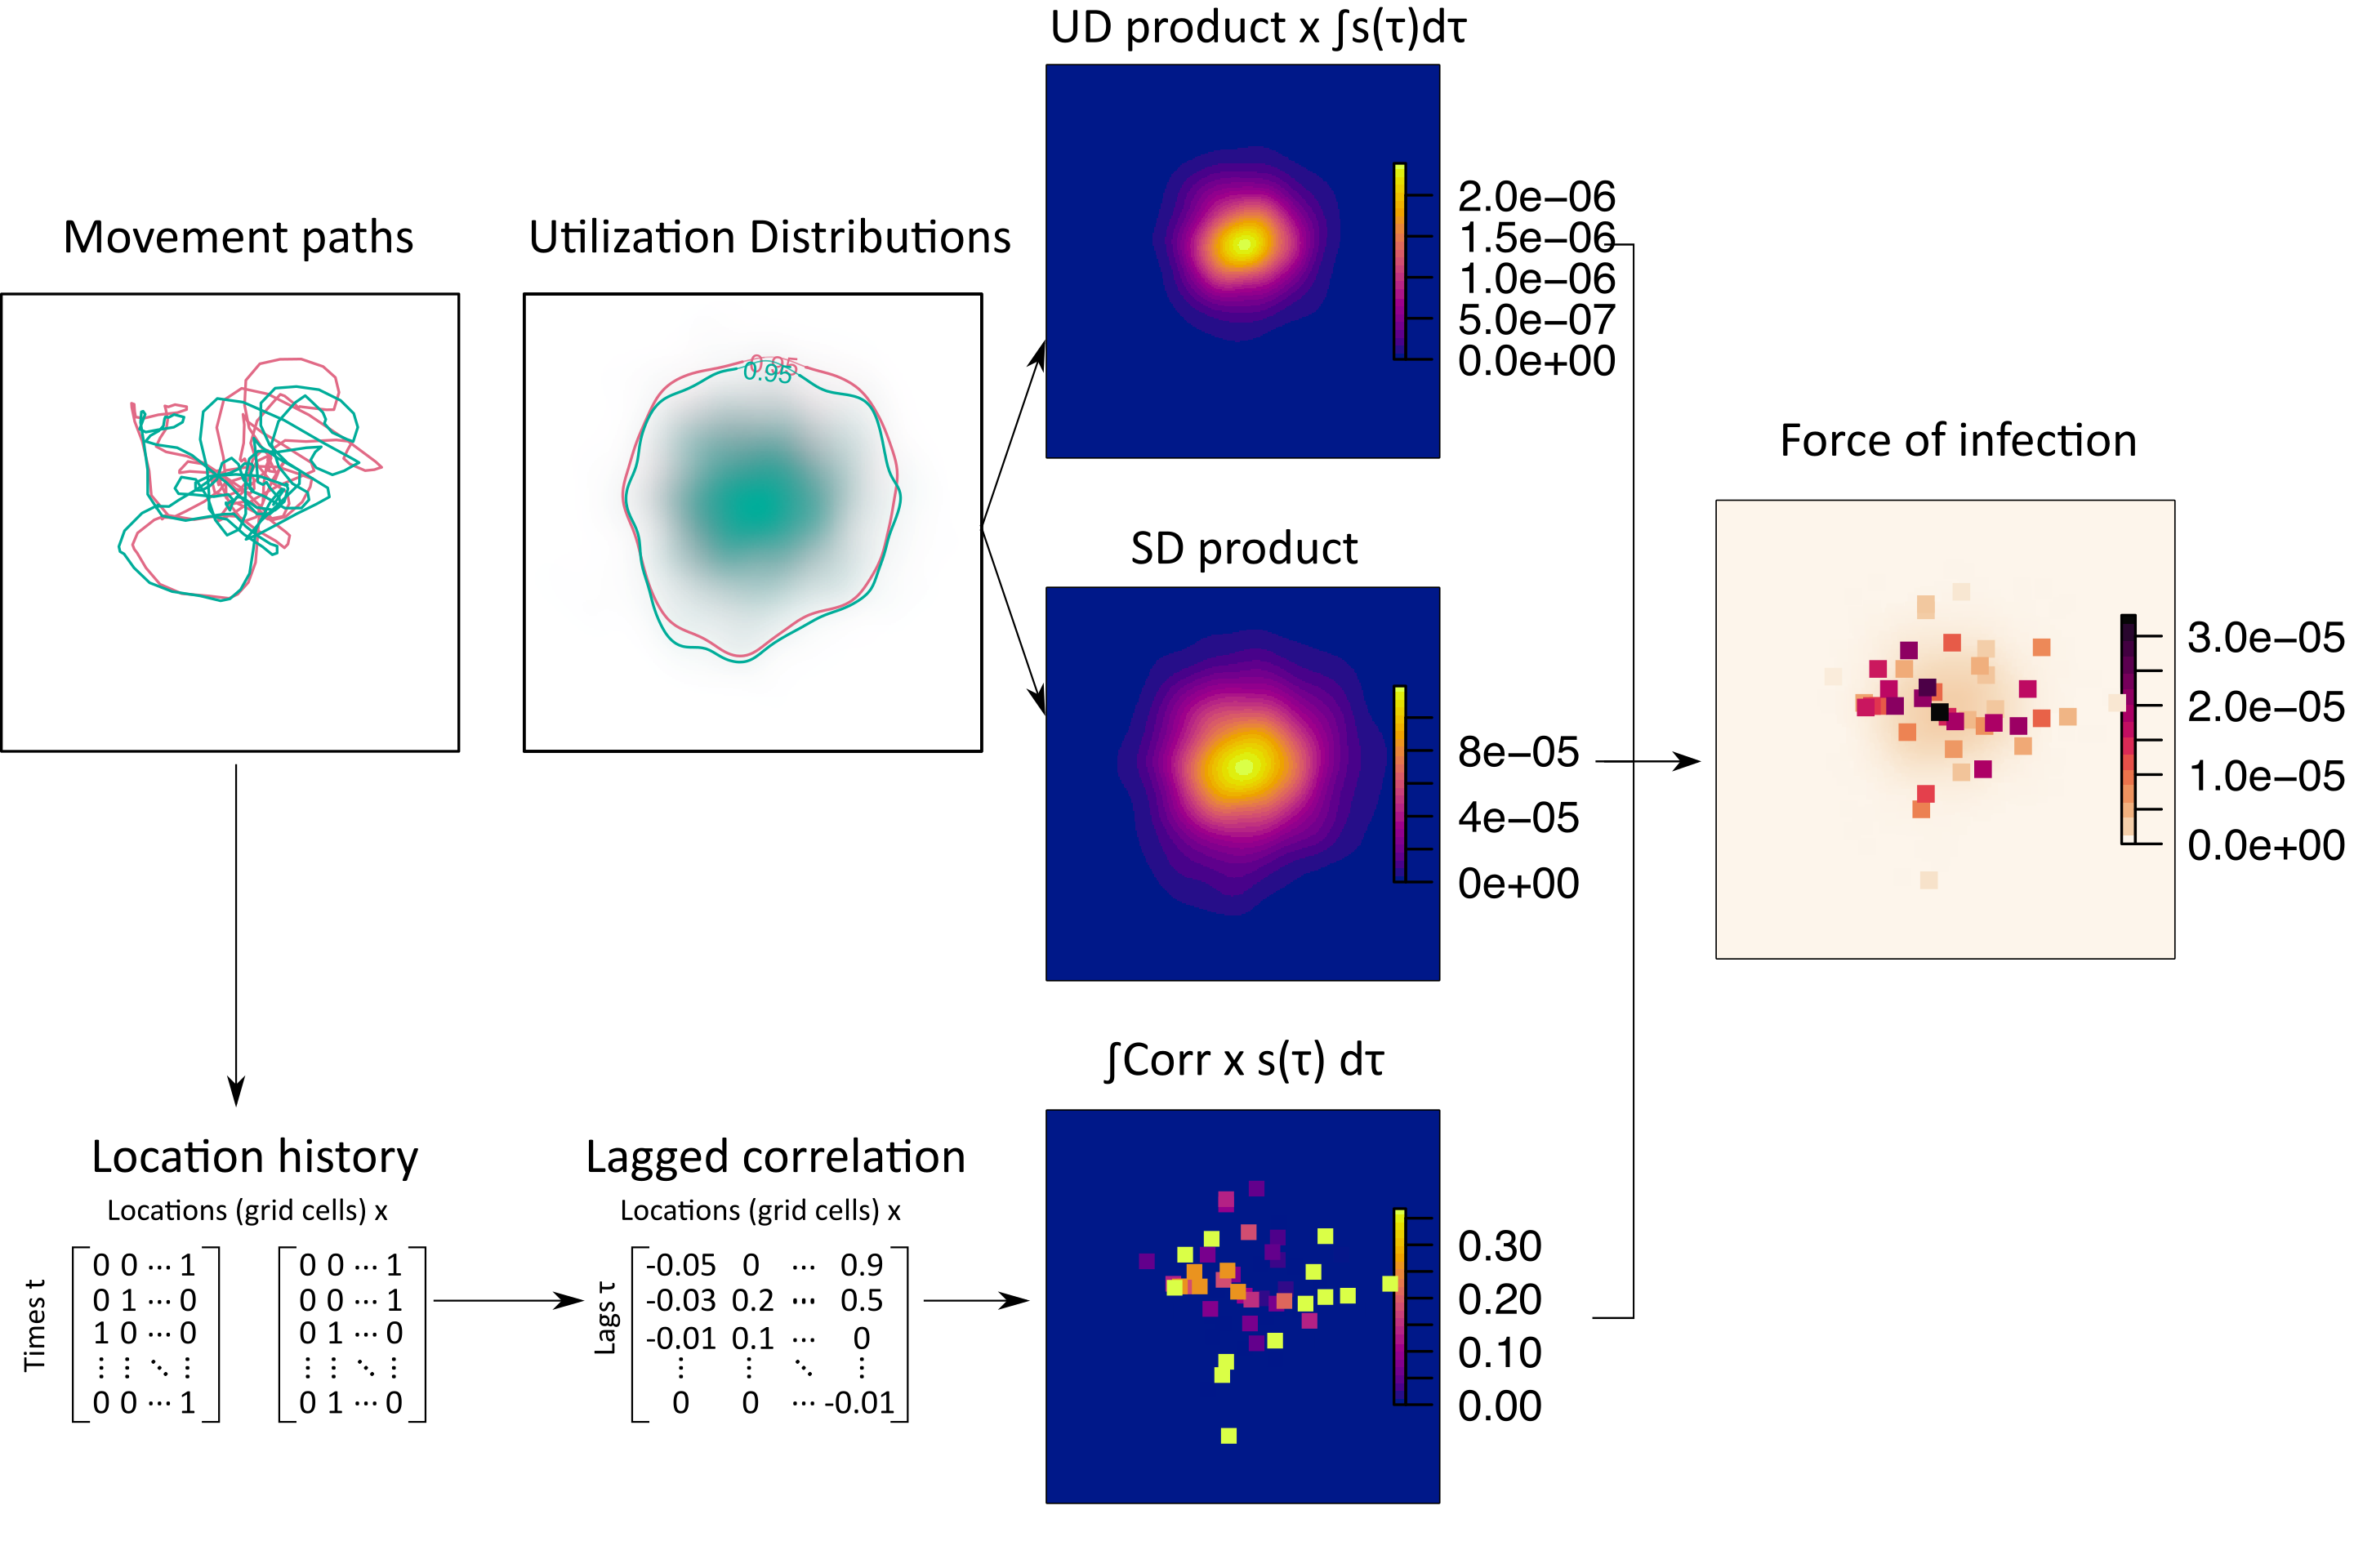
\includegraphics[width=\textwidth]{figures/steps_diagram.png}
     \caption{Flow diagram illustrating how to estimate the spatial force of infection (FOI) from empirical movement data using the PMoveSTIR framework. Starting from position data, we estimate individual utilization distributions, and use them to estimate the product of the UDs and their standard deviations (SDs). In addition, individual position histories are used to estimate the pairwise temporal cross-correlation in space use at each cell (e.g., the correlation term in equation \ref{eq:stationary_cor}). All three elements are combined and scaled by epidemiological parameters to obtain a spatially explicit, pairwise, directional FOI.} %Note that here and in the manuscript we do not spatially interpolate the correlation surface. We therefore provide a conservative view of how correlation contributes to landscape-level FOI.}
  \label{fig:steps}
 \end{figure}

\begin{figure}
    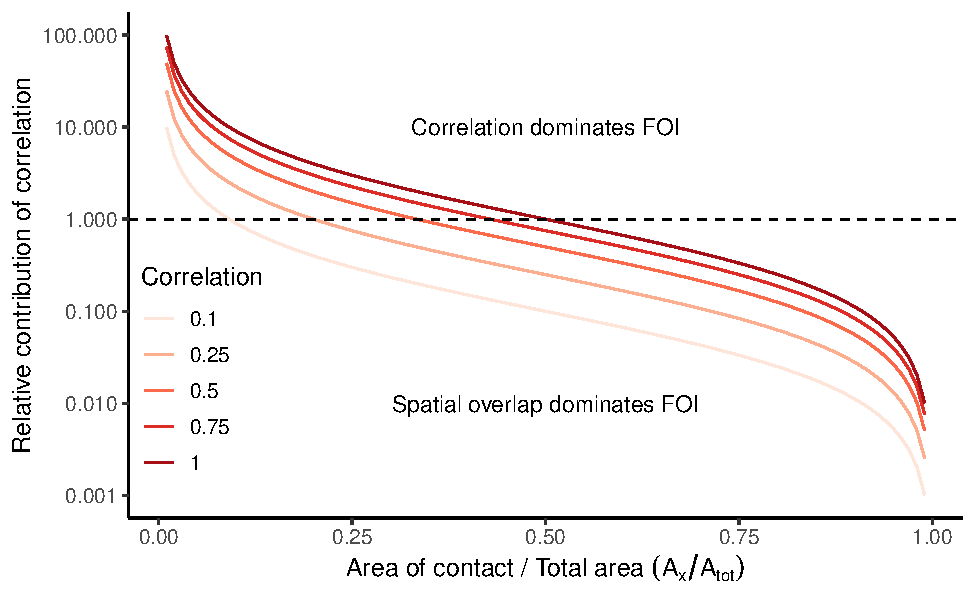
\includegraphics[width=\textwidth]{figures/correlation_analytical_figure.pdf}
    \caption{Relationship between the relative contribution of correlation in space use to pairwise force of infection (FOI) and the relative area of contact. This analytical relationship is derived in equation \ref{eq:uniform_direct} assuming direct contact.}  %When the relative area of contact is small relative to the total area over which animals can move (e.g., $<$ 10\%), even weakly non-independent movements can significantly increase FOI relative to spatial overlap.}
    \label{fig:analytical_corr}
\end{figure}

\begin{figure}
    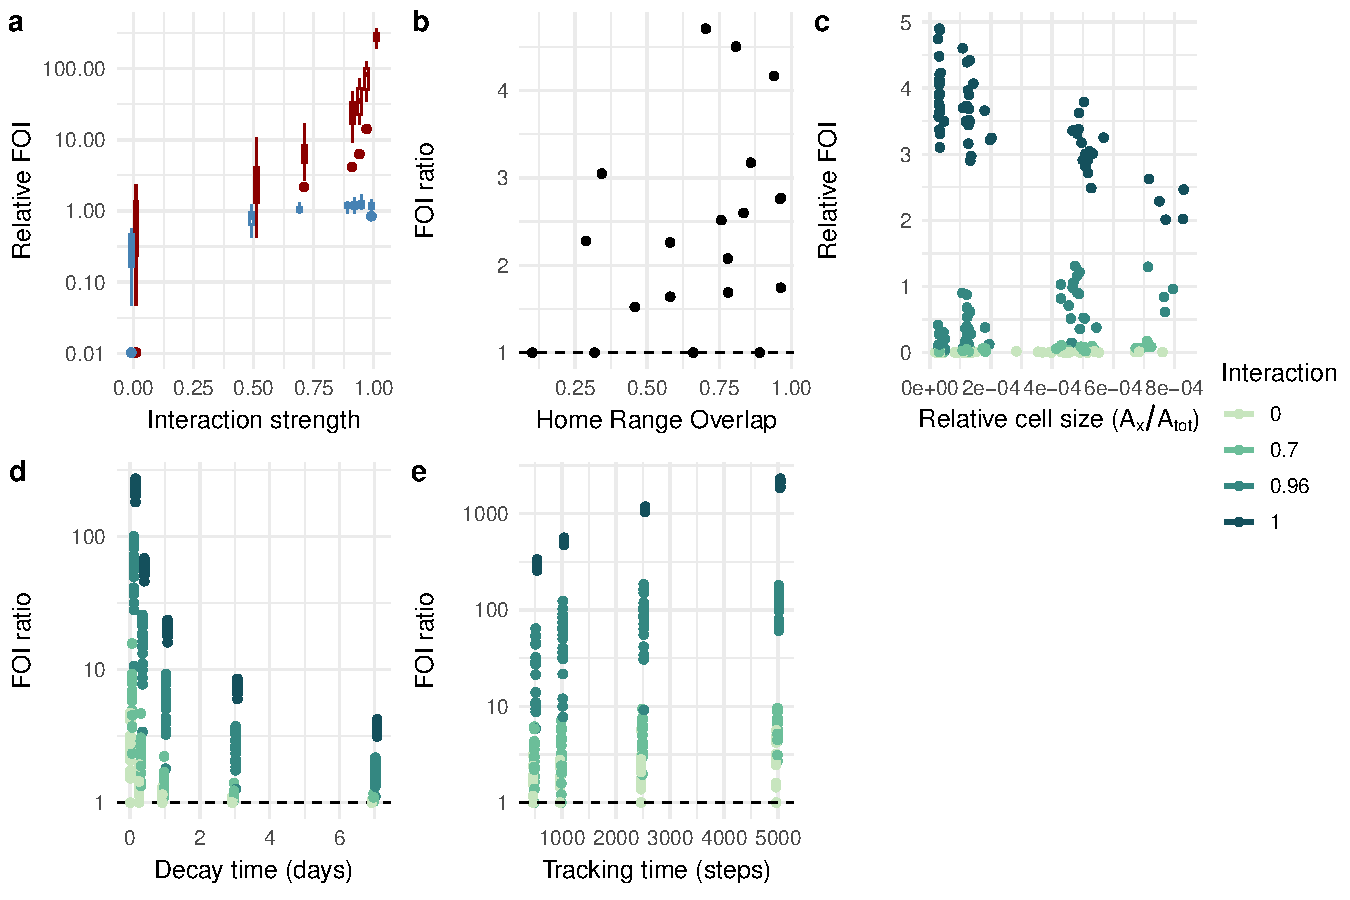
\includegraphics[width=\textwidth]{figures/sim_results.pdf}
    \caption{\small Analysis of force of infection (FOI) values estimated from simulated trajectories. \textbf{a)} Relative FOI as a function of attraction strength between individuals, calculated considering only spatial overlap (blue), or incorporating correlation in space use (red);  \textbf{b)} Ratio of FOI estimated with and without correlation for independent trajectories, as a function of home range overlap (as measured by the Bhattacharyya coefficient);   \textbf{c)} Relative FOI as a function of the size of individual cells, relative to the combined home range of both individuals; \textbf{d)} FOI ratio as a function of mean time to decay (assuming exponential decay); \textbf{e)} FOI ratio as a function of total duration of the simulations. Longer simulations would produce correlation values at more cells. In c-e, darker shades indicate greater interaction strength between individuals. }
  \label{fig:simresults}
\end{figure}

\begin{figure}
    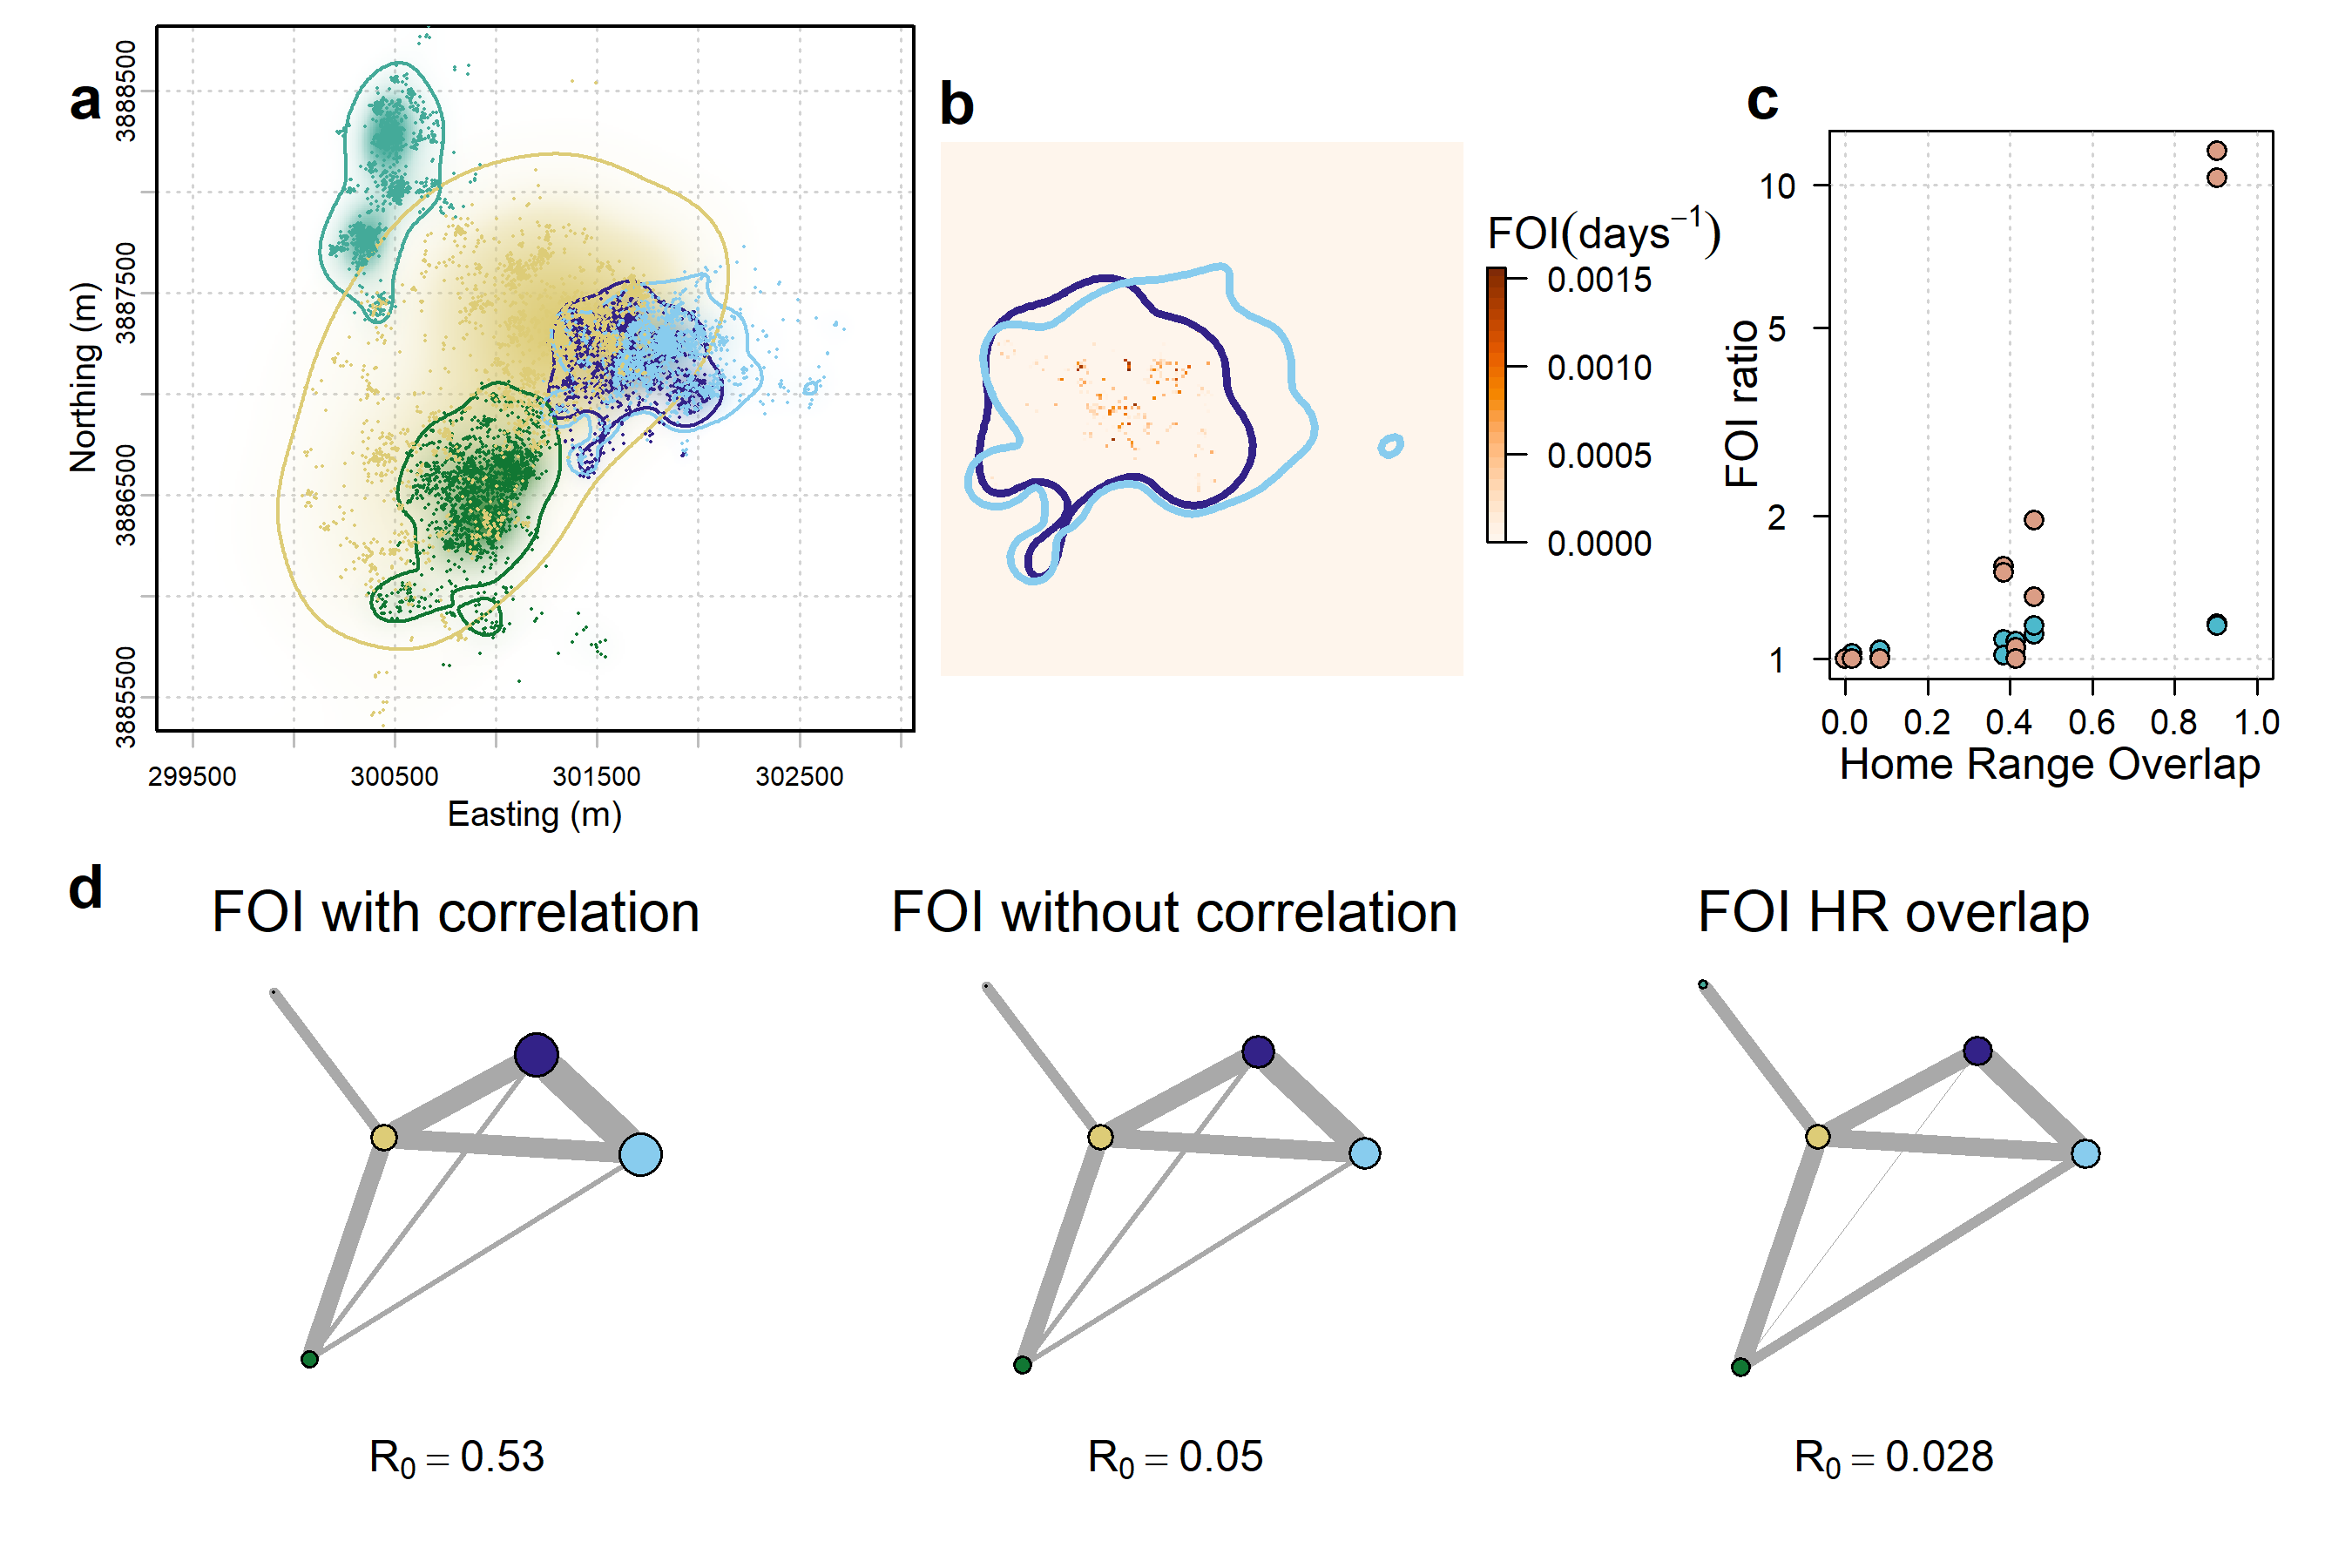
\includegraphics[width=\textwidth]{figures/deer_results.png}
    \caption{\small Application of the PMoveSTIR framework to movements of white-tailed deer in TN, USA. \textbf{a)} Home ranges of five individuals with different degrees of overlap. The points show the GPS locations, and the lines are the boundaries of the home ranges, estimated as the region that contains 95\% of the utilization distribution density. \textbf{b)} Detail of the home ranges of the two individuals that overlapped the most. The color surface shows the estimated FOI, highlighting how accounting for temporal correlation creates a heterogeneous surface of disease transmission risk with distinct hotspots. \textbf{c)} Ratio of FOI values calculated with versus without correlation as a function of home range overlap for a pathogen with short environmental persistence like SCV2 (orange dots) and a pathogen with long persistence like CWD (blue triangles). \textbf{d)} Transmission networks created with the PMoveSTIR framework including correlation (left), without correlation (middle), and using the home range overlap (right). The size of the nodes represents the cumulative FOI experienced by each individual, and the width of the edges represents the pairwise FOI. We show only one direction here, but values were similar in both directions within a pair. Sizes and widths have the same scale in all three networks. $R_0$ values should only be interpreted with respect to each other and not in absolute value.}
  \label{fig:empiricalres}
\end{figure}


\end{document}
